\begin{BlueBox}
    \vskip-1cm
    \begin{block}{\BHead{Background}}
        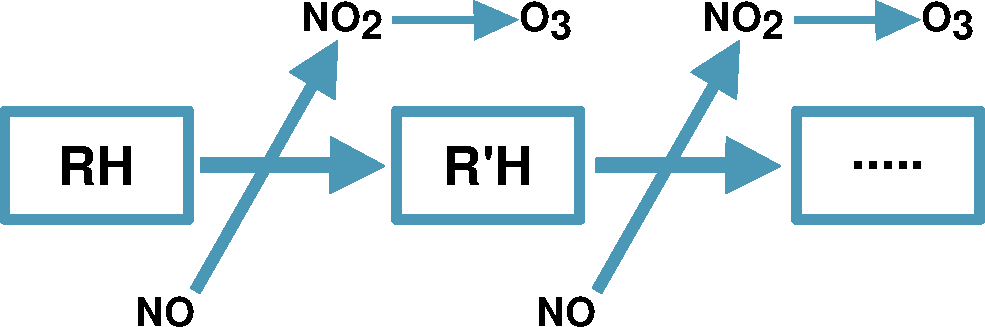
\includegraphics[width=\textwidth]{VOC_Oxidation} \vspace{5mm}
        \begin{itemize}
            \item Ozone is produced from photochemistry of emitted VOC and \ce{NO_x}, VOC is the ``fuel'' and \ce{NO_x} the ``catalyst''. \vspace{10mm}
            %\item Climate change will increase surface temperatures. \vspace{5mm}
            \item Temperature drives surface ozone in many areas. \vspace{10mm}
            \item Temperature influences ozone production by \vspace{4mm}
                \begin{itemize}
                    \item increasing BVOC emissions from vegetation, 
                    \item increasing reaction rates of many atmospheric chemistry processes.  \vspace{10mm}
                \end{itemize}
            \item Is increased BVOC emissions or increased chemistry more important for increasing ozone with temperature? \vspace{-3mm}
            \item Do chemical mechanisms used in models reproduce the relationship between ozone and temperature across \ce{NO_x} gradients? \vspace{10mm}
        \end{itemize}
    \end{block}
\end{BlueBox}
